\documentclass[12pt]{article}
\usepackage[margin=2cm]{geometry}
\usepackage{amsmath,amssymb,amsthm}
\usepackage{graphicx}
% For subfigure environments
\usepackage{subcaption}
\usepackage[framemethod=tikz]{mdframed}
\usepackage{booktabs}

% Optional: for [H] specifier
\usepackage{float}

\graphicspath{ {./images/} }


\title{\vspace{2cm}
    \Huge \textbf{Heuristic Optimization Techniques}\\[2cm]
    \LARGE Report 2
    \vspace{10cm}
    
    \large Aksinia Vorobeva, 12044614  \\ Marcel Korinek, 12220824
    }

\begin{document}

\maketitle


\pagebreak

\section{Problem Description}
\begin{mdframed}[
    linecolor=black,
    linewidth=1.5pt,
    roundcorner=5pt,
    backgroundcolor=blue!5,
    userdefinedwidth=\textwidth,
]
\textbf{Selective Capacitated Fair Pickup and Delivery Problem (SCF-PDP)}

\vspace{0.7em}
\textbf{Graph model:}  
Complete directed graph $G = (V, A)$, where:
\begin{itemize}
    \item $V$ contains the depot as well as all pickup and drop-off locations.
    \item $A = \{(u,v) : u, v \in V, u \neq v\}$ represents travel arcs.
    \item Each arc $(u,v)$ has an associated distance  
    \[
        a_{u,v} = \left\lceil \sqrt{(x_u - x_v)^2 + (y_u - y_v)^2} \right\rceil,
    \]
    where $(x_u, y_u)$ are the coordinates of location $u$.
\end{itemize}

\vspace{0.5em}
\textbf{n Customer requests:}   
For each request $i \in \{1, \dots, n\}$ there are:
\[
v_i^{\uparrow} \in V \quad \text{(pickup location)}, \qquad
v_i^{\downarrow} \in V \quad \text{(drop-off location)}.
\]

The solution must serve at least $\gamma \le n$ of them.

\vspace{0.5em}
\textbf{Vehicles:}  
A fleet $K$ of $n_K$ identical vehicles is available, each with capacity $C$ and starting/ending at the depot.

\vspace{0.7em}
\textbf{Feasible solution:}  
A solution consists of a route $R_k$ for each vehicle $k \in K$, where $R_{k,i}$ denotes the $i$-th stop. Each solution must satisfy:
\begin{itemize}
    \item Vehicle load never exceeds capacity $C$
    \item Each served request is fully handled by a single vehicle
    \item At least $\gamma$ requests are served in total
\end{itemize}

The travel duration of route $R_k$ is
\[
d(R_k)
= a_{\text{depot}, R_{k,1}}
+ a_{R_{k,|R_k|}, \text{depot}}
+ \sum_{(u,v)\in R_k} a_{u,v}.
\]

\vspace{0.5em}
\textbf{Fairness measure:}  
We use the Jain fairness index:
\[
J(R)
=
\frac{\left(\sum_{k \in K} d(R_k)\right)^2}
{\,n_K \cdot \sum_{k \in K} d(R_k)^2\, }.
\]

\vspace{0.7em}
\textbf{Objective:}  
Minimize the total travel duration penalized by unfairness:
\[
\sum_{k \in K} d(R_k)
\;+\;
\rho \cdot (1 - J(R)),
\]
where $\rho$ controls the trade-off between efficiency and fairness.

\end{mdframed}

\subsection{Experimental Setup}
All experiments were made on a machine with a AMD Ryzen 7 9800X3D and 32 RAM, running Windows 11 and Python 3.13.9.

We tested every algortihm on all of the instances with size 50 and 100. For every non-deterministic algorithm we made at least three runs in order to increase the significance of the results.

For each experiment, the relevant algorithm configurations are provided in the corresponding chapter.

\section{Description of Algorithms}

Every algorithm shares five input parameters: \emph{customers}, \emph{vehicles}, \emph{to$\_$fulfilled}, \emph{rho} and \emph{output$\_$statistic}. 

\vspace{0.6em}
\textbf{Customers.}

The input parameter \emph{customers} is a list of \texttt{Customer} objects, each customer contains the relevant information for each request:

\begin{itemize}
    \item a unique identifier
    \item a pickup location and a drop-off location, both represented as \texttt{Point} objects
    \item the amount of goods to be transported
\end{itemize}

A \texttt{Point} object contains the coordinates, the point type (depot, pickup, drop-off),
and the quantity of goods associated with it (if the point type is pickup, then  the quantity of goods is positive for pickups, if it is drop-off, then the quantity is negative).

\vspace{0.6em}
\textbf{Vehicles.}

The most important parameter is \emph{vehicles}, which is also our choice of a solution representation for this problem. It is a list of \texttt{Vehicle} objects.
Each vehicle maintains the following:
\begin{itemize}
    \item its capacity
    \item its current load and position
    \item its route, stored as a sequence of \texttt{Point} objects
    \item its accumulated path length
    \item a load-history tracing the load after each visited point
\end{itemize}
Together, the set of vehicles encodes the full multi-vehicle our routing solution, including which requests are served and in what order.

\vspace{0.6em}
\textbf{Minimum Requests to Serve.}

The parameter \emph{to\_fulfill} describes the minimum number of requests to
be served.

\vspace{0.6em}
\textbf{Fairness Weight \boldmath$\rho$.}

The parameter \emph{rho} is the fairness weight in the objective function.
It is passed to the \texttt{ObjectiveTracker}, which evaluates
\[
\text{Objective}
=
\sum_{k} d(R_k)
\;+\;
\rho \cdot (1 - J(R)),
\]
and updates values efficiently using delta evaluation.

\vspace{0.6em}
\textbf{Output Statistics.}

The parameter \texttt{output\_statistic} is irrelevant for the functionality of the algorithms, as it is only relevant for the experimental evaluation and result analysis. We save the collection of detailed performance data using the \texttt{Statistic} class,
including:
\begin{itemize}
    \item the objective value over time
    \item fairness values over time
    \item total route duration over time
    \item the number of iterations performed
\end{itemize}

\vspace{1em}
\textbf{Algorithm output.}

Ultimately, at the end of the algorithm, we receive:

\begin{itemize}
    \item a file in .txt format with the final solution to the problem
    \item statistical data
    \item a graphical representation of the solution (see Figure~\ref{fig:graph_rep_sa})
\end{itemize}


\begin{figure}[H]
    \centering
    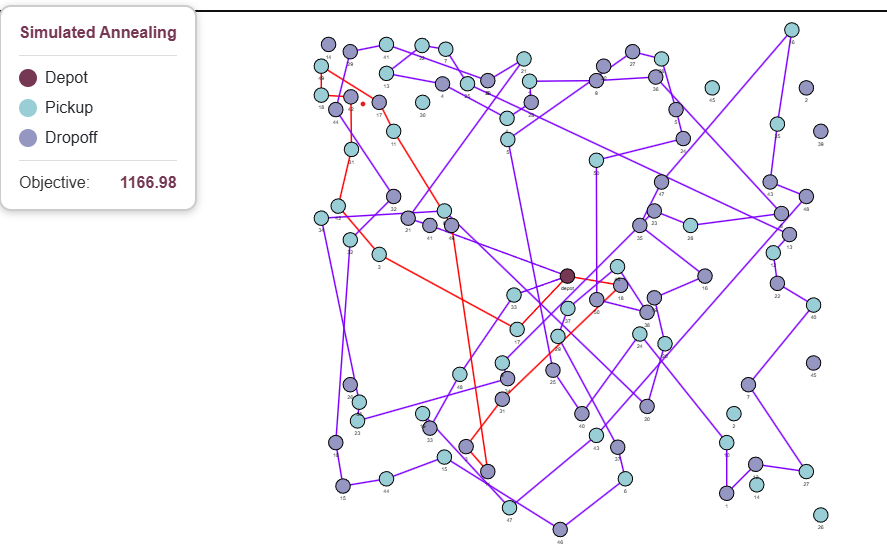
\includegraphics[width=\linewidth]{graphics/output_1.png}
    \caption{Graphical representation of SA output}
    \label{fig:graph_rep_sa}
\end{figure}

\subsection{Genetic Algorithm}


The proposed solution method is based on a Genetic Algorithm (GA), an evolutionary metaheuristic that iteratively improves a population of candidate solutions through biologically inspired operators. 

\bigskip

The Genetic Algorithm is controlled by a set of problem-specific and algorithmic parameters, summarized below.

\begin{itemize}
    \item \textbf{customers}: List of all \texttt{Customer} objects.
    \item \textbf{vehicles}: List of a given number of empty \texttt{Vehicle} objects.
    \item \textbf{to\_fulfilled}: Minimum number of customer requests that must be fulfilled.
    \item \textbf{rho}: Fairness weight.
    \item \textbf{s}: Selection pressure.
    \item \textbf{t\_max}: Maximum number of generations (iterations).
    \item \textbf{population\_size}: Number of individuals in the population.
    \item \textbf{num\_elites}: Number of elite individuals preserved during replacement.
    \item \textbf{selection\_method}: Parent selection strategy.
    \item \textbf{tournament\_size}: Number of individuals competing in each tournament (only relevant if tournament selection is the chosen selection method).
    \item \textbf{tournament\_replace}: Sets whether an individual can be chosen multiple times for a tournament (only relevant if tournament selection is the chosen selection method).
    \item \textbf{recombination\_rate}: Probability of applying crossover to a selected pair.
    \item \textbf{recombination\_weights}: Operator-specific weights.
    \item \textbf{recombination\_samples}: Number of tries to insert a pickup point and a dropoff point randomly in a vehicle path (relevant for submethods of the recombination)
    \item \textbf{mutation\_rate}: Probability of mutating an offspring.
    \item \textbf{mutation\_weights}: Operator-specific weights.
    \item \textbf{output\_statistic}: Boolean value indicating if the more details regarding the run should be returned.
\end{itemize}

\pagebreak


The overall procedure consists of the following main phases:

\begin{enumerate}
    \item \textbf{Initialization}: Generation of an initial population of feasible solutions.
    \item \textbf{Evaluation}: Computation of the objective value (fitness) for each individual.
    \item \textbf{Selection}: Choice of parent individuals for Recombination based on their fitness.
    \item \textbf{Recombination}: Creation of new offsprings by combining solution parts from selected parents.
    \item \textbf{Mutation}: Random modification of offsprings to maintain diversity and explore new regions of the search space.
    \item \textbf{Replacement}: Construction of the next generation by replacing the old population by the offsprings while potentially also preserving elite individuals.
\end{enumerate}

Steps 2 to 6 are repeated until a maximum number of iterations is reached or the algorithm exceeds a runtime of 10 minutes.



Each of the phases listed above is described in detail in the subsequent chapters.

\subsubsection{Initialization}

Each individual of the initial population is generated using a fast constructive procedure. For every customer request, a vehicle is selected uniformly at random, and the corresponding pickup and drop-off nodes are appended to the current route of that vehicle. This procedure is computationally efficient and yields a roughly balanced initial assignment of customers across all vehicles. The resulting solutions are not necessarily of high quality. However, this is acceptable, as the primary objective of the initialization phase is to provide diverse and feasible starting points for the evolutionary search rather than near-optimal solutions.


\subsubsection{Evaluation}

The evaluation phase assigns a fitness value to each individual in the population and consists of two main steps.

\paragraph{Fitness Transformation.}
Since the considered problem is a minimization problem, while the Genetic Algorithm operates on a maximization of fitness, the objective values are first transformed accordingly. Let $c_i$ denote the objective value of individual $i$ and let
\[
c_{\max} = \max_{j \in P} c_j + 1
\]
be a constant larger than any objective value in the current population $P$. The raw fitness of individual $i$ is then computed as
\[
f_i = c_{\max} - c_i .
\]
By construction, all fitness values are strictly positive and a smaller objective value results in a larger fitness.

\paragraph{Linear Scaling.}
To control the selection pressure and avoid premature convergence, a linear scaling of the raw fitness values is applied. Let $f_{\max}$, $f_{\text{avg}}$, and $f_{\min}$ denote the maximum, average, and minimum fitness in the population, respectively. The scaled fitness $\hat{f}_i$ is obtained as
\[
\hat{f}_i = a f_i + b ,
\]
where the scaling coefficients $a$ and $b$ are chosen such that
\[
\hat{f}_{\text{avg}} = f_{\text{avg}}, \qquad
\hat{f}_{\max} = s \cdot \hat{f}_{\text{avg}},
\]
with $s > 1$ being a user-defined scaling factor. Solving this system yields
\[
a = \frac{(s-1) \hat{f}_{\text{avg}}}{f_{\max} - \hat{f}_{\text{avg}}}, \qquad
b = f_{\text{avg}} - a \hat{f}_{\text{avg}} .
\]

In order to guarantee non-negative scaled fitness values, the coefficients are further adjusted if $\hat{f}_{\min} < 0$ by enforcing $\hat{f}_{\min} = 0$. 
In this case, the parameters are recomputed as
\[
a = \frac{\hat{f}_{\text{avg}}}{\hat{f}_{\text{avg}} - f_{\min}}, 
\qquad
b = a \hat{f}_{\text{avg}} - \hat{f}_{\text{avg}},
\]

The resulting scaled fitness values are finally used in the subsequent selection phase.
This linear scaling mechanism preserves the ranking of individuals while regulating the difference between the best and average fitness, thereby balancing exploration and exploitation during the evolutionary search.

\bigskip

Right after the evaluation phase, the solution of the best individual of the recently evaluated population is compared to the best found solution so far. This ensures that at the end of the whole algorithm always the best solution of all generations is returned.



\subsubsection{Selection}

The selection phase determines which individuals of the current population are chosen as parents for the recombination. Individuals with higher fitness values are given a higher probability of being selected, thereby implementing the principle of survival of the fittest while still preserving stochasticity to maintain population diversity. If a number of elites is specified, this will be considered by choosing only \texttt{population\_size} - \texttt{num\_elites} parents. Two selection mechanisms are implemented: roulette-wheel selection and tournament selection.

\paragraph{Roulette-Wheel Selection.}
In roulette-wheel (fitness-proportionate) selection, each individual $i$ is assigned a selection probability proportional to its fitness value $f_i$. Let $P$ be the current population and $F = \sum_{j \in P} f_j$ the sum of all fitness values. The probability of selecting individual $i$ is given by
\[
p_i = \frac{f_i}{F}.
\]
Parents are then sampled from the population according to this discrete probability distribution. As a consequence, individuals with higher fitness are more likely to be selected, while lower-quality individuals still retain a non-zero chance of contributing to the next generation.

\paragraph{Tournament Selection.}
In tournament selection, a set of $k$ individuals (the tournament size) is drawn uniformly at random from the population, either with or without allowing duplicates (toggled by the replacement parameter). The individual with the highest fitness among the selected contenders is declared the winner of the tournament and is chosen as a parent. This procedure is repeated until the required number of parents has been selected.

The tournament size $k$ directly controls the selection pressure: larger values of $k$ increase the probability that highly fit individuals are selected, while smaller values promote diversity.

Both selection strategies preserve the ranking induced by the fitness values, but differ in their stochastic behavior and selection pressure. The choice between them and the tuning of their parameters significantly influence the balance between exploration and exploitation in the evolutionary process.


\subsubsection{Recombination}

The recombination phase generates new candidate solutions (offsprings) by combining structural components of two parent individuals. Let $Q_s$ denote the list of selected parents. Parents are processed sequentially in pairs. For each pair $(p_1, p_2)$, recombination is applied with probability \texttt{recombination\_rate}. If recombination is not applied, both parents are copied unchanged to the offspring population.

If recombination is triggered, one recombination operator is chosen randomly from a predefined set of operators, where the probability of choosing a specific operator is controlled by the user-defined weights \texttt{recombination\_weights}. Depending on the chosen operator, either one or two children may be produced. If only one child is returned, the same operator is applied again with reversed parent roles to obtain a second offspring. If the number of selected parents is odd, the last unpaired parent is copied directly into the offspring population.


\paragraph{Customer-Based Recombination.}
In customer-based recombination, a child is initialized as a copy of the first parent. Then, for each customer, a decision is made independently with a fixed probability (set to $0.8$) whether the customer should be kept from the first parent. All customers that are not selected to be kept are removed from the child solution by deleting both their pickup and drop-off nodes from the corresponding vehicle route.

The missing customers are reinserted according to the order induced by the second parent. For each missing customer, the algorithm first checks in which vehicle the customer appears in the second parent. If such a vehicle exists, the customer is inserted into the corresponding vehicle of the child; otherwise, the customer is assigned to the currently shortest vehicle route. In both cases, insertion is performed by a stochastic insertion heuristic that tries several random pickup and drop-off positions and keeps the most promising candidates with respect to the objective function.

After all missing customers have been reinserted, a repair procedure is applied to eliminate duplicates, resolve infeasibilities, and enforce the minimum number of fulfilled requests. This operator produces exactly one child.

\paragraph{Vehicle-Based Recombination.}
In vehicle-based recombination, two children are created simultaneously. First, copies of both parents are made. The vehicle list of the first child is randomly permuted. Then, for each vehicle position $k$, the vehicles of the two children are swapped with probability $0.5$. This produces offsprings that inherit entire vehicle routes from both parents.

Since this operation may create duplicate or missing customer assignments, a repair procedure is subsequently applied to both children to restore feasibility and to ensure that each customer appears at most once and that at least \texttt{to\_fulfilled} requests are served.

\paragraph{Stochastic Insertion.}
Both recombination operators rely on a stochastic insertion subroutine for placing a customer into a given vehicle route. For a customer with pickup node $p$ and drop-off node $d$, random pairs of insertion positions $(i,j)$ with $i<j$ are sampled, where $p$ is inserted after position $i$ and $d$ after position $j$. For each sampled pair, the resulting path length and its impact on the global objective function are estimated. Among all tried candidates, the best \texttt{samples} insertion positions are kept.

These candidates are then tested in increasing order of predicted objective value. The first insertion that yields a valid route is accepted. If none of the candidates is feasible, a fallback strategy inserts the pickup just before the final depot and the drop-off immediately after the pickup, followed by a reordering step to restore consistency.

\paragraph{Repair Procedure.}
After recombination, offspring solutions may contain customers multiple times or may violate feasibility conditions. The repair procedure first scans all customers and removes duplicates by keeping the occurrence in the shorter vehicle route and deleting the other.

If the solution already satisfies the minimum number of fulfilled requests, it is accepted. Otherwise, all currently unassigned customers are collected. While the solution is infeasible and fewer than \texttt{to\_fulfilled} insertion attempts have been made, customers are selected randomly from this set and inserted into the currently shortest route using the stochastic insertion procedure.

If no unassigned customers remain but the solution is still infeasible, the entire child is reset to a copy of the first parent, ensuring that recombination never produces an unusable individual.


\subsubsection{Mutation}

The mutation phase introduces random local changes into offspring solutions in order to preserve diversity and to reduce the risk of premature convergence. Let $Q_r$ denote the population after recombination. Each individual is mutated independently with probability \texttt{mutation\_rate}. If an individual is selected for mutation, one mutation operator is drawn randomly from a predefined set, where the probability of choosing a specific operator is controlled by the user-defined weights \texttt{mutation\_weights}. If no mutation is applied, the individual is passed unchanged to the next population.

\paragraph{Swap Mutation.}
Swap mutation modifies the assignment of two randomly chosen customer requests. Two distinct customers are sampled uniformly at random. Let $v_1$ and $v_2$ denote the vehicles currently serving the first and second customer, respectively. Three cases are distinguished:

\begin{itemize}
\item If both customers are unassigned, the attempt is discarded.
\item If exactly one customer is assigned to a vehicle, that customer is removed from its vehicle and replaced by the unassigned customer, inserting the pickup and drop-off nodes of the previously unassigned customer at the same positions.
\item If both customers are assigned, their pickup and drop-off nodes are exchanged between the two vehicles.
\end{itemize}

After performing the exchange or replacement, all affected vehicle routes are checked for feasibility. If the modified routes are valid, the mutated individual is accepted. Otherwise, the attempt is rejected and repeated. This process is carried out up to a fixed number of attempts, after which the original individual is returned if no valid mutation could be generated.

\paragraph{Move Mutation.}
Move mutation relocates a single customer from its current vehicle to a different vehicle. First, a customer that is currently assigned to some vehicle is selected uniformly at random. Its current vehicle is identified, and another vehicle is chosen uniformly at random as the target.

Random insertion positions for the pickup and drop-off nodes are selected in the target vehicle route, excluding the depot positions. The customer is removed from its original vehicle and inserted into the target vehicle at the chosen positions. If both modified vehicle routes are feasible after the move, the mutation is accepted. Otherwise, the attempt is rejected and repeated. As for swap mutation, only a limited number of trials is performed before reverting to the original individual.

\paragraph{Neighborhood-Based Mutation.}
Neighborhood-based mutation applies a local improvement step rather than a purely random change. One neighborhood structure is selected uniformly at random from a predefined set, including exchange, pickup relocation, drop-off relocation, remove-and-append, and move operations. Starting from the current solution, a neighboring solution is generated according to the chosen structure using a first-improvement strategy guided by the objective function and the fairness parameter $\rho$.

If a strictly better neighboring solution is found, the individual is replaced by this improved solution. Otherwise, the individual remains unchanged. This operator therefore acts as an intensification mechanism that exploits the local structure of the search space.

\subsubsection{Replacement}

The replacement phase constructs the population of the next generation by combining elite individuals (if there are any) from the current population with the newly generated offsprings. This preserves the size of the population throughout every iteration.

\bigskip

After the replacement, the new population continues with the evaluation phase. 

\subsubsection{Parameter Tuning}

The performance of a Genetic Algorithm strongly depends on the choice of its parameters. Therefore, a systematic parameter tuning process was carried out using the automatic configuration tool \textit{irace}. Tuning was performed separately for problem instances of size 50 and 100 from the set of training instances, as these instance classes differ significantly in computational difficulty and runtime behavior.

\paragraph{Tuning Setup.}
For the instance set of size 50, the tuning scenario was defined with a maximum of 300 experiments and a confidence level of $0.95$. The tuning process executed the algorithm through a batch script, which forwarded the parameter values proposed by \textit{irace} to the main solver via the command line.

Each run of the algorithm returned only the final objective value, which was used by \textit{irace} as the performance measure to be minimized.


\paragraph{Tuned Parameters.}
The following parameters were included in the tuning process:

\begin{itemize}
\item Number of generations $t_{\max}$
\item Population size
\item Selection pressure $s$
\item Selection method (roulette-wheel or tournament)
\item Tournament size and replacement policy
\item Recombination operator weights
\item Mutation operator weights
\item Number of elite individuals
\item Number of recombination samples
\item Recombination rate
\item Mutation rate
\end{itemize}


\paragraph{Instance-Specific Tuning.}
Tuning was carried out independently for instances of size 50 and 100. This separation was necessary because larger instances impose stricter time limits, which changes the trade-off between population size, number of generations, and operator complexity. By tuning both instance classes separately, parameter configurations could be adapted to the different computational budgets and problem characteristics.

\paragraph{Tuned Parameter Configurations.}
These resulting configurations, shown below for each instance size, were then fixed and used for all subsequent experimental evaluations. This ensures that the reported results reflect well-calibrated algorithmic behavior rather than arbitrary parameter choices.



\begin{table}[H]
    \centering
    \caption{Resulting GA parameter configurations for instances of size 50 and 100.}
    \begin{tabular}{lcc}
        \toprule
        \textbf{Parameter} & \textbf{Size 50} & \textbf{Size 100} \\
        \midrule
        Number of generations, $t_{\max}$ & 170 & 134 \\
        Population size & 62 & 76 \\
        Selection pressure, $s$ & 1.0625 & 1.5719 \\
        Selection method & tournament & tournament \\
        Tournament size & 62 & 35 \\
        Tournament replace & False & False \\
        Recombination weights & [ 0.7411,  0.1901] & [0.7883, 0.4033] \\
        Mutation weights & [0.3749, 0.3587, 0.4831] & [0.7198, 0.5541, 0.537] \\
        Number of elite individuals & 24 & 32 \\
        Recombination samples & 176 & 10 \\
        Recombination rate & 0.4257 & 0.9743 \\
        Mutation rate & 0.1647 & 0.4273 \\
        \bottomrule
    \end{tabular}
    \label{tab:ga_parameters}
\end{table}


\begin{figure}[H]
    \centering
    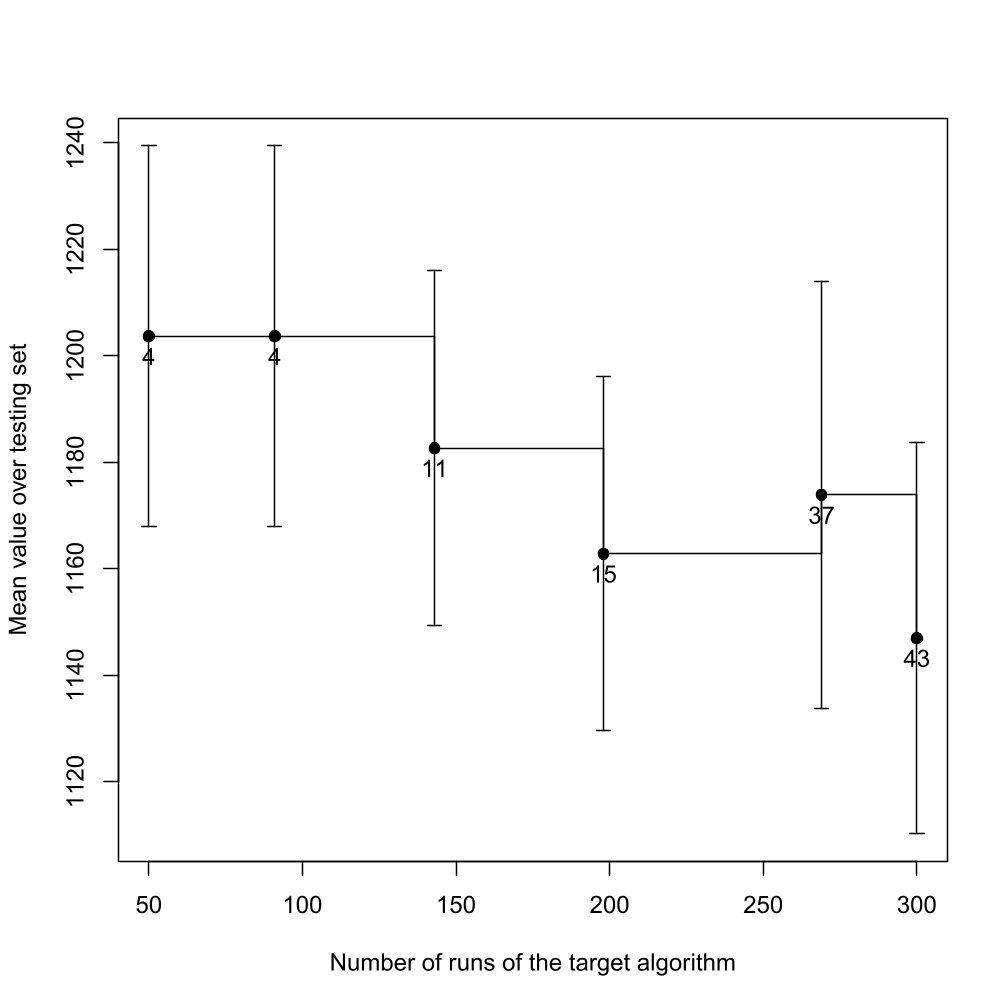
\includegraphics[width=0.48\linewidth]{graphics/irace_ga_50.jpg}
    \hfill
    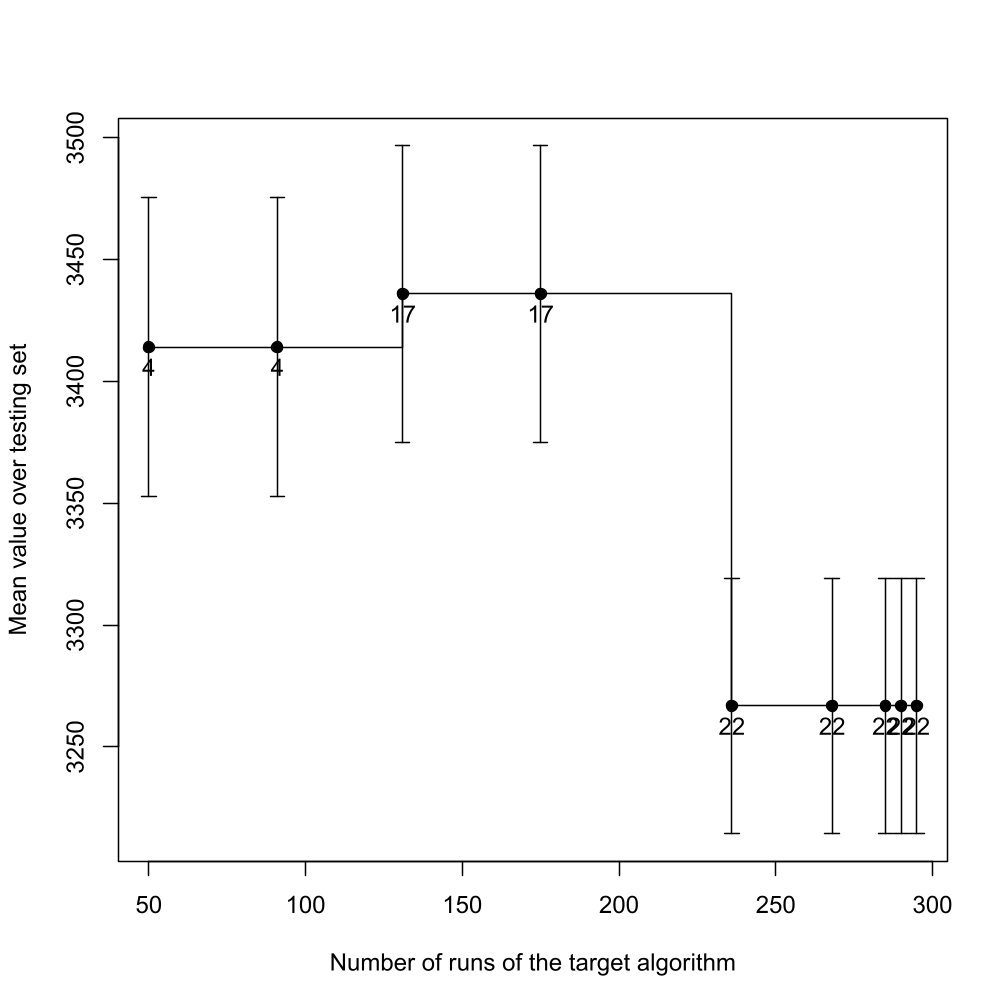
\includegraphics[width=0.48\linewidth]{graphics/irace_ga_100.jpg}
    \caption{Configuration Quality Over Time for Instances of Size 50 (left) and 100 (right).}
    \label{fig:irace_convergence}
\end{figure}

Figure~\ref{fig:irace_convergence} shows how the quality of the best parameter configuration improved as the number of tuning runs increased.


\subsubsection{Evolution of Solution Quality and Fairness}

Figure~\ref{fig:ga_obj_over_time} illustrates the improvement of the solution quality over time. The most significant progress is achieved during the initial iterations, after which the objective value change gets smaller and converges towards a stable value.

\begin{figure}[H]
    \centering
    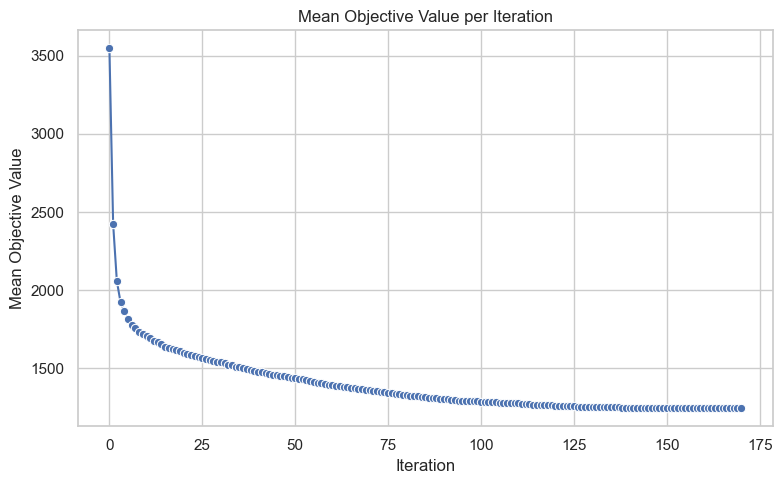
\includegraphics[width=0.7\linewidth]{graphics/ga_obj_over_time.png}
    \caption{Mean Objective Value Over Iterations for 50 Customers (GA)}
    \label{fig:ga_obj_over_time}
\end{figure} 

The evolution of fairness over iterations is presented in Figure~\ref{fig:ga_fairness_over_time}. Although the fairness slightly decreases, it remains above 0.975, which is still a very high fairness value.

\begin{figure}[H]
    \centering
    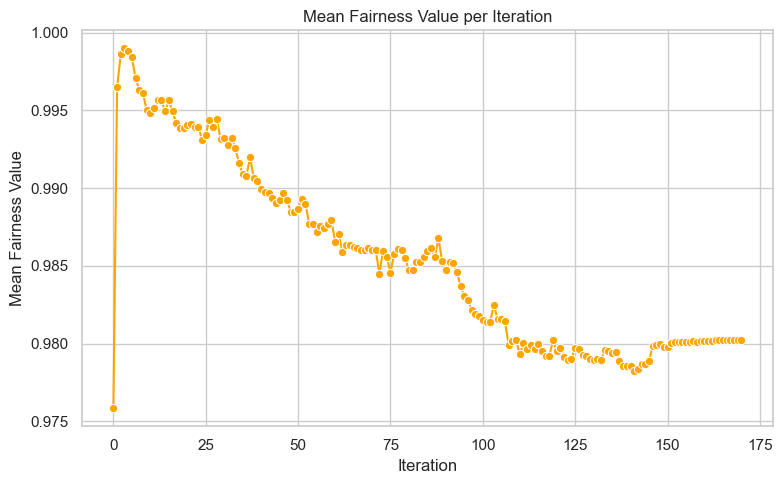
\includegraphics[width=0.7\linewidth]{graphics/ga_fairness_over_time.png}
    \caption{Mean Fairness Value Over Iterations for 50 Customers (GA)}
    \label{fig:ga_fairness_over_time}
\end{figure} 

\pagebreak



\subsection{Ant Colony Optimization}

As an alternative metaheuristic approach, we decided to implement the Ant Colony Optimization algorithm, which is inspired by the behavior of real ant colonies. Each ant colony constructs a feasible solution using indirect communication between ants through pheromone trails.

In our proposed solution each ant incrementally constructs a feasible pickup-and-delivery route for one associated vehicle under capacity, precedence, and fulfillment constraints. So, the number of ants in the colony is the same as the number of vehicles. The algorithm iteratively improves the solution by reinforcement of promising edges using updates of pheromones and evaporation to avoid premature convergence.

\bigskip

The ACO algorithm contains the following problem-specific and algorithmic parameters:

\begin{itemize}
    \item \textbf{customers}: List of all \texttt{Customer} objects.
    \item \textbf{initial\_ solution}: List of a given number of empty \texttt{Vehicle} objects.
    \item \textbf{to\_fulfilled}: Minimum number of customer requests that must be fulfilled.
    \item \textbf{rho}: Fairness weight.
    \item \textbf{graph}: Weighted directed graph representing the transportation network.
    \item \textbf{n\_colonies}: Number of ant colonies constructed per iteration. (iterations).
    \item \textbf{alpha}: Influence of pheromone intensity on decision making.
    \item \textbf{beta}: Influence of heuristic desirability (inverse distance).
    \item \textbf{evaporation}: Pheromone evaporation rate.
    \item \textbf{obj\_ name}: Selected fairness objective (min–max, Gini, or Jain).
    \item \textbf{output\_statistic}: Boolean value indicating if the more details regarding the run should be
returned.
    \item \textbf{visualization}: Boolean flag that enables real-time visualization of pheromone dynamics (see Figure~\ref{fig:aco_vis}).
\end{itemize}

\begin{figure}[H]
    \centering
    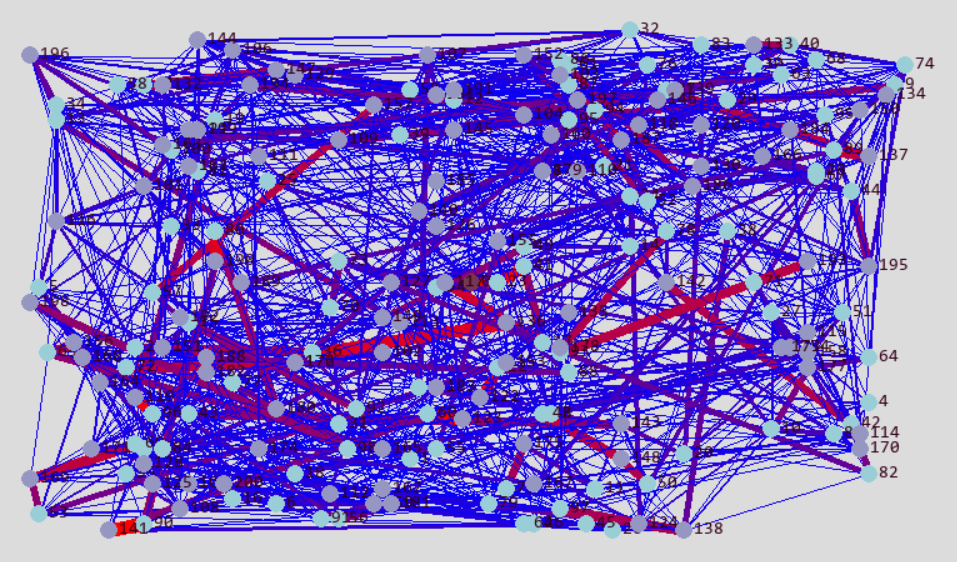
\includegraphics[width=0.7\linewidth]{graphics/aco_vis.png}
    \caption{Real-time visualization of pheromone dynamics}
    \label{fig:aco_vis}
\end{figure} 

The overall procedure consists of the following main phases:

\begin{enumerate}
    \item \textbf{Initialization}: Initialization of pheromone values and ant colonies.
    \item \textbf{Solution Construction}: Construction of feasible routes by ants.
    \item \textbf{Evaluation}: Computation of the objective value for the colony's solution.
    \item \textbf{Pheromone Update}: Evaporation and reinforcement of pheromone trails.
    \item \textbf{Termination}: Repetition until a fixed number of iterations is reached.
\end{enumerate}

Each phase is described in detail below.

\subsubsection{Initialization}

At the start of the ACO algorithm every edge of the graph becomes a small uniform pheromone value and some properties that are not affecting the solution quality but used for the real-time visualization.

For each iteration the colony starts with new ants. Every ant is associated with one vehicle and constructs one feasible route. The pickup nodes are initially available to all ants, whereas the drop-off nodes become available to one ant after the corresponding pickup has been visited by this ant. It ensures precedence feasibility and allows each customer to be fulfilled by a single ant.

\subsubsection{Solution Construction}

Working as cooperative colony ants construct a complete solution step by step. Every ant is responsible for one vehicle. At each step every active ant select feasible successor node, which are constrained by:

\begin{itemize}
    \item The current load of vehicle
    \item Pickup-Delivery precedence
    \item Remaining fulfillment requirements
\end{itemize}

Let the ant be located at node $i$, then the set of feasible successors for an ant location is denoted by $N_i$. The probability of moving from node $i$ to node $j \in N_i$ is defined as
\[
p_{ij}
=
\frac{\tau_{ij}^{\alpha} \cdot \eta_{ij}^{\beta}}
{\displaystyle \sum_{k \in N_i} \tau_{ik}^{\alpha} \cdot \eta_{ik}^{\beta}},
\]

where $\tau_{ij}$ denotes the pheromone intensity on edge $(i,j)$ and
$\eta_{ij}$ is the heuristic desirability given by
\[
\eta_{ij} = \frac{1}{d_{ij}},
\]
where $d_{ij}$ is the  distance between nodes $i$ and $j$.

At every step, all the ants choose the next node for themselves. The algorithm compares these decisions, yielding the best improvement with respect to the global fairness objective. The step with the best objective is selected and executed, while the same node is removed from the feasible sets of the other ants. This cooperation ensures that the constructed solution does not violate the given constraints and respects fairness. 

Once one ant has reached all feasible nodes for selection, it becomes inactive. When all ants completed their routes, each vehicle returns to the depot.

\subsubsection{Evaluation}

After the construction is completed, the qualities of the solutions are evaluated based on the selected objective function. The objective values of all colonies are stored and then used for best global tracking and reinforcement of pheromones.

The best colony that is found in the current iteration is compared to the best global solution, and if the improvement is detected, the best global solution is updated accordingly.

\subsubsection{Pheromone Update}

The pheromone update is done using a rank-based Ant System strategy.
First, pheromone evaporation is applied to all edges:
\[
\tau_{ij} \leftarrow (1 - \rho)\,\tau_{ij}.
\]

The colonies are then ranked according to their objective values.
Only the top $w$ colonies (in our case the best half of colonies) deposit pheromone, with rank $r = 0$ denoting the best colony.

Objective values are normalized as following
\[
q_r
=
\frac{f_r - f_{\min}}
{f_{\max} - f_{\min} + \varepsilon},
\]
where $f_r$ is the objective value of colony $r$, and
$f_{\min}$ and $f_{\max}$ are the minimum and maximum objective values among all colonies.

For a colony of rank $r$, the pheromone increment deposited on edge $(i,j)$ is defined as
\[
\Delta \tau_{ij}^{(r)}
=
\frac{(w - r)\, Q \, q_r}
{1 + \varepsilon \, L},
\]
where $L$ is the route length of the corresponding vehicle and
$\varepsilon$ is a small positive constant.

The total pheromone update is given by
\[
\tau_{ij} \leftarrow \tau_{ij}
+ \sum_{r=0}^{w-1} \Delta \tau_{ij}^{(r)}.
\]

\subsubsection{Termination}

The algorithm terminates if the fixed number of iterations is executed.
 At the end the best solution found across all iterations is returned.

\subsubsection{Parameter Tuning}

The well-known property of Ant Colony Optimization is a high sensitivity to the choice of its algorithmic parameters that are controlling the balance between exploration and exploitation.

Unlike the Genetic Algorithm, whose parameters we tuned using the automatic configuration tool \textit{irace}, the parameters of the ACO algorithm were selected using a custom racing-based procedure with used of scipy.stats library.

\paragraph{Tuning Setup.}
Parameter tuning was performed on the set of training instances with 50 customers using jain coefficient for the objective function.
For each candidate parameter configuration, the ACO algorithm was executed on multiple training instances, and the resulting objective values were recorded. Over repeated runs the mean objective value was used as the performance measure for the minimization.

Previously evaluated configurations were always cached to reduce redundant computations and reused whenever possible.

\paragraph{Parameter Space.}
The tuning procedure explored a discrete parameter space defined as the Cartesian product of the following parameter domains:
\begin{itemize}
    \item Number of colonies $n_{\text{col}} \in \{5, 10, 20\}$
    \item Pheromone influence $\alpha \in \{0.5, 1.0, \dots, 3.0\}$
    \item Heuristic influence $\beta \in \{2.0, 3.0, \dots, 6.0\}$
    \item Evaporation rate $\rho \in \{0.02, 0.06, \dots, 0.20\}$
\end{itemize}

\paragraph{Racing Procedure.}
The evaluation of configurations was executed step by step on an increasing number of instances. After each instance a non-parametric Friedman test was applied to detect statistically significant performance differences among the surviving configurations. If it was no significant difference all instances became survivors, in other case if the Friedman test indicated significance at $\alpha = 0.05$, pairwise
one-sided Wilcoxon signed-rank tests were performed between the best performing configuration and the remaining candidates.
Then the Bonferroni correction was used to control for multiple comparisons and decrease the probability of Type 1 error.
Configurations that were found to be statistically inferior were eliminated from the race.

The conditions of the elimination process were:

\begin{itemize}
    \item a single configuration remained
    \item all training instances had been processed
\end{itemize}


\paragraph{Tuned Parameter Configurations.}
The racing-based tuning procedure did not converge to a single dominant configuration, the result of the tuning for ACO algorithm was represented by a small set of statistically indistinguishable parameter settings.
All surviving configurations are reported in Table~\ref{tab:aco_parameters}.

\begin{table}[H]
    \centering
    \caption{Resulting ACO parameter configurations obtained from the racing procedure.}
    \begin{tabular}{cccc}
        \toprule
        \textbf{$n_{\text{col}}$} & \textbf{$\alpha$} & \textbf{$\beta$} & \textbf{Evaporation $\rho$} \\
        \midrule
        20 & 0.50 & 6.00 & 0.14 \\
        20 & 0.50 & 6.00 & 0.02 \\
        20 & 0.50 & 6.00 & 0.18 \\
        10 & 0.50 & 6.00 & 0.02 \\
        10 & 0.50 & 6.00 & 0.06 \\
        20 & 0.50 & 5.00 & 0.10 \\
        20 & 0.50 & 5.00 & 0.14 \\
        20 & 0.50 & 6.00 & 0.06 \\
        20 & 0.50 & 6.00 & 0.10 \\
        20 & 1.00 & 5.00 & 0.02 \\
        20 & 1.00 & 6.00 & 0.02 \\
        20 & 1.00 & 6.00 & 0.06 \\
        \bottomrule
    \end{tabular}
    \label{tab:aco_parameters}
\end{table}


\paragraph{Discussion of Tuning Results.}
Across surviving configurations of parameters we can see several consistent patterns.

First, this is a relatively low value of the pheromone influence parameter $\alpha$ (either $0.5$ or $1.0$), combined with large values of the heuristic influence parameter $\beta$ ($5.0$ or $6.0$).
This indicates that the algorithm benefits from a strong emphasis on heuristic information, while relying not so much on pheromone trails. This behavior is consistent for our problem, because it is logical that distance-based decisions often lead to feasible and efficient routes, especially in early construction phases.

Second, the majority of configurations with high performance use a large number of colonies ($n_{\text{col}} = 20$), although some configurations with $n_{\text{col}} = 10$ also survive the racing procedure.

Third, no dominating evaporation rate $\rho$ was detected.
Low evaporation values ($\rho = 0.02$) and higher values ($\rho = 0.18$) appear among the surviving configurations probably due to the rank-based update of pheromones. 


\paragraph{Final Parameter Selection.}
As a result the parameter combination
\[
n_{\text{col}} = 20, \quad \alpha = 0.5, \quad \beta = 6.0, \quad \rho = 0.10
\]
was selected for all subsequent experimental evaluations.

\subsubsection{Evolution of Solution Quality and Fairness}

Figure~\ref{fig:ga_obj_over_time} shows how the solution quality improves throughout the iterations. 

\begin{figure}[H]
    \centering
    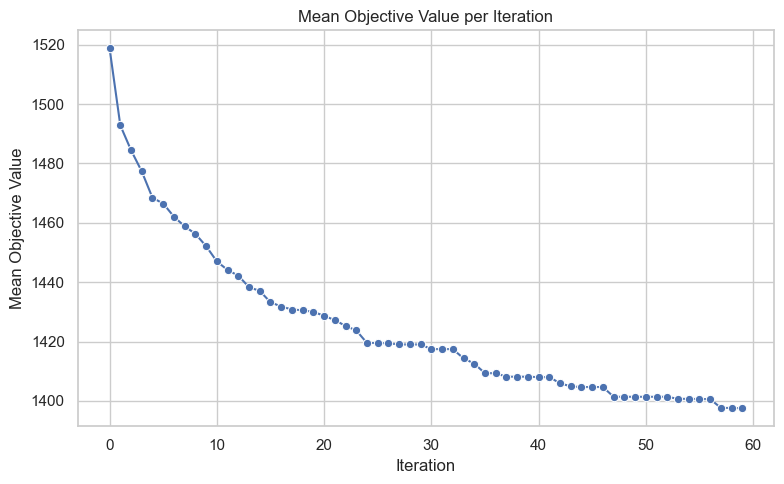
\includegraphics[width=0.7\linewidth]{graphics/aco_obj_over_time.png}
    \caption{Mean Objective Value Over Iterations for 50 Customers (ACO)}
    \label{fig:aco_obj_over_time}
\end{figure} 

Figure~\ref{fig:ga_fairness_over_time} illustrates the evolution of the fairness value over the course of the iterations. Overall, the fairness metric exhibits an increasing trend, rising from an initial value of approximately 0.89 to about 0.94.

\begin{figure}[H]
    \centering
    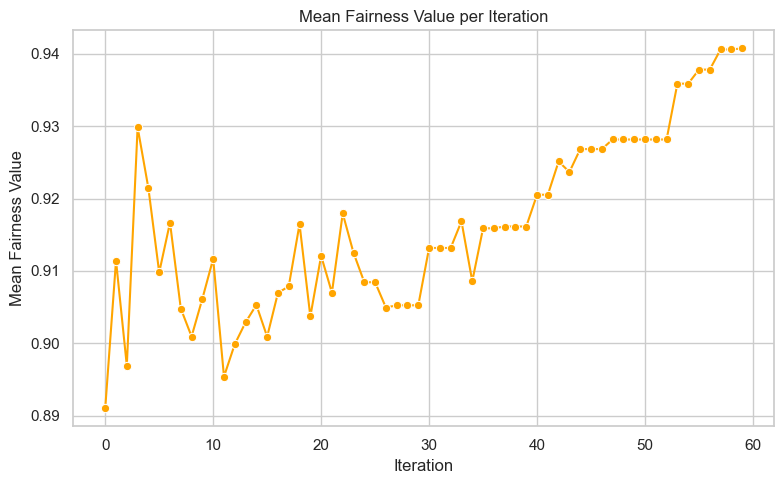
\includegraphics[width=0.7\linewidth]{graphics/aco_fairness_over_time.png}
    \caption{Mean Fairness Value Over Iterations for 50 Customers (ACO)}
    \label{fig:aco_fairness_over_time}
\end{figure} 


\pagebreak

\subsection{Impact of Different Fairness Measures}

To analyze the impact of fairness metric on the solution quality we replaced Jain fairness index $J(R)$ in the objective function by two proposed alternative fairness measures:

\begin{itemize}
    \item max--min fairness and
    \item inverted Gini coefficient
\end{itemize}

The resulting solutions were obtained using the ACO algorithm in 50 customer instances and compared in terms of objective value, route length balance, customer distribution across routes, and fairness represents the chosen measure (see Figure~\ref{fig:comp_meas}).

\paragraph{Objective Value.}
On the first plot we can clearly see that the average objective function for each instance differs only slightly. All three measures allow us to obtain almost the same result.

\paragraph{Route Length Balance.}
As expected, max--min fairness usually achieves the strongest control over route length imbalance,
leading to the smallest ratio between the longest and shortest routes. But for some instances the balance can be even worse in comparison to other fairness measures. It can be related to the strictness of this measure that can limit the algorithm’s ability to minimize the total travel distance on the one hand and get balanced solution on the other.
There is no significant difference on balance between Gini coefficient and Jain fairness.

\paragraph{Number of Stops Over the Routes.}
The average balance of number of stops (served customer locations) almost completely corresponds to the balance of length between the shortest and longest routes.

\begin{figure}[H]
    \centering
    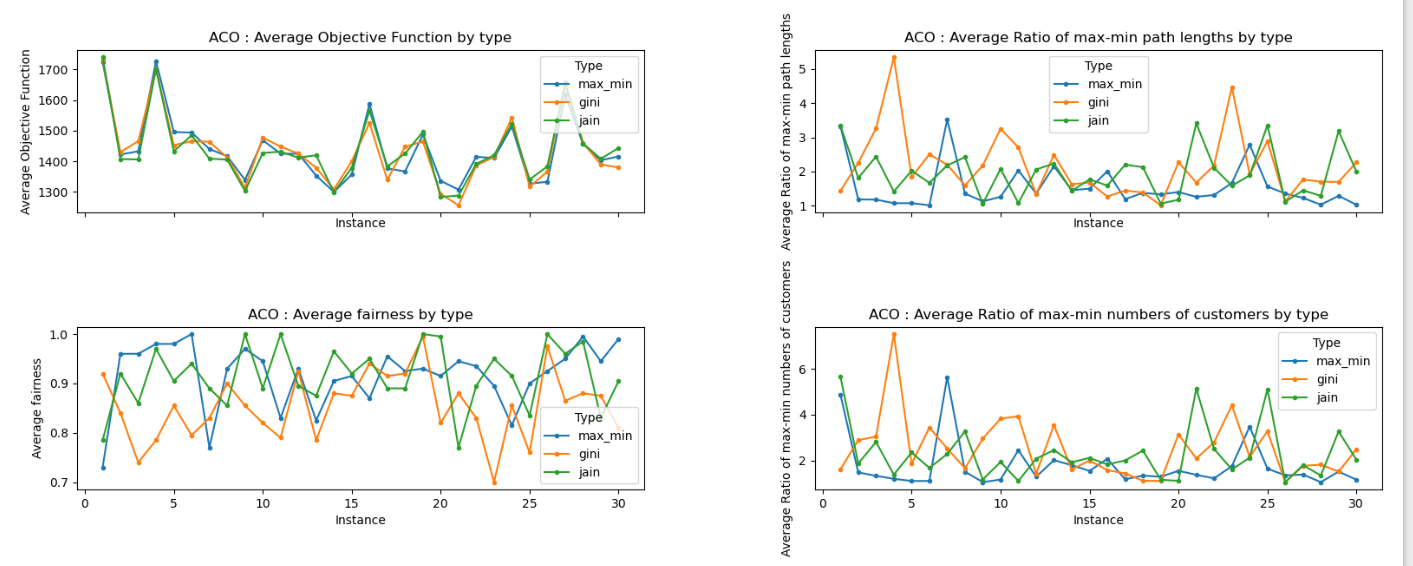
\includegraphics[width=1\linewidth]{graphics/comp_meas.png}
    \caption{Comparison of fairness measures}
    \label{fig:comp_meas}
\end{figure} 


The lower left plot on Figure~\ref{fig:comp_meas} shows that the Jain fairness index consistently has lower
average fairness values compared to
max--min fairness and the inverted Gini coefficient.
This behavior can be explained by the structural properties.

\paragraph{Max--Min Fairness.}
Max--min fairness is defined as
\[
M = \frac{\min_{k \in K} d(R_k)}{\max_{k \in K} d(R_k)},
\]
where $d(R_k)$ denotes the length of route $R_k$.
This measure depends only on the extreme routes.
So, the optimization process focuses on equalizing the shortest and longest
routes, when the intermediate routes are not explicitly constrained.

\paragraph{Inverted Gini Coefficient.}
The inverted Gini coefficient is defined as
\[
G = 1 -
\frac{
\sum_{k' \in K} \sum_{k'' \in K}
\left| d(R_{k'}) - d(R_{k''}) \right|
}{
2 n_K \sum_{k' \in K} d(R_{k'})
},
\]
where $n_K$ is the number of routes.
This measure considers inequality across \emph{all} pairs of routes, but aggregates these
in a global manner.
The imbalances must be smoothed out, producing relatively high and stable
fairness.

\paragraph{Jain Fairness Index.}
Jain fairness is defined as
\[
J(R) =
\frac{\left( \sum_{k \in K} d(R_k) \right)^2}
{n_K \sum_{k \in K} d(R_k)^2}.
\]
Unlike max--min and Gini fairness, Jain fairness is more sensitive to small variations among routes are amplified, which leads to lower fairness scores when
the route lengths are not nearly identical.




\pagebreak

\subsection{Comparison Between GA and ACO}

This subsection analyzes the performance of GA and ACO.

\subsubsection{Experimental Results}

The experimental results show that GA consistently produces lower objective
values than ACO for both instances of size 50 and 100. This behavior can be observed
in the boxplots (Figures~\ref{fig:comparison_ga_aco_50} and \ref{fig:comparison_ga_aco_100}) and in the per-instance bar charts (Figures~\ref{fig:comparison_ga_aco_50_per_instance} and \ref{fig:comparison_ga_aco_100_per_instance}), where GA dominates ACO across all
tested instances. The visual analysis already suggests a clear advantage of GA
over ACO in terms of solution quality.


Regarding computational efficiency, ACO demonstrates a clear advantage over GA. As illustrated in the right parts of Figures~\ref{fig:comparison_ga_aco_50} and \ref{fig:comparison_ga_aco_100}, ACO consistently requires significantly less CPU time across all instances. While GA provides higher solution quality, the lower execution time of ACO suggests it may be more suitable for time-sensitive applications where a rapid solution is required.

\begin{figure}[H]
    \centering
    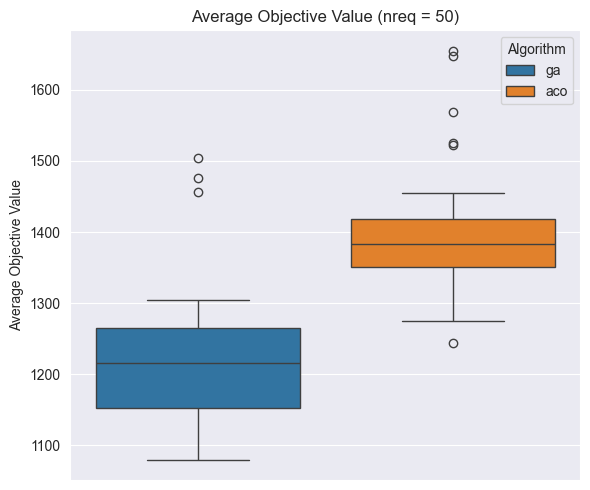
\includegraphics[width=0.42\linewidth]{graphics/comparison_ga_aco_50_obj.png}
    \hfill
    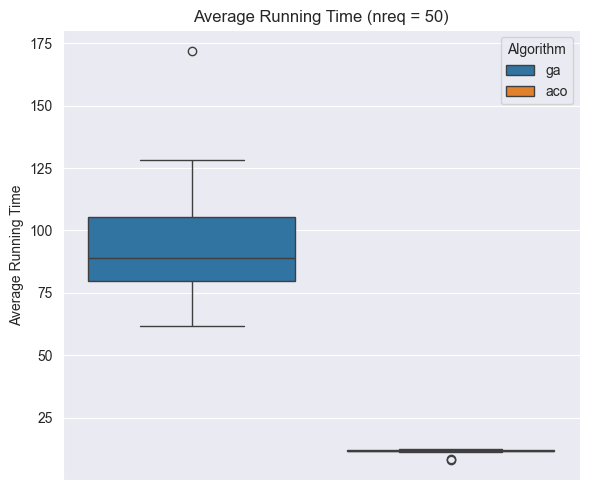
\includegraphics[width=0.42\linewidth]{graphics/comparison_ga_aco_50_time.png}
    \caption{Comparison GA vs. ACO: Average Objective Function and Run Time for
50 Customers}
    \label{fig:comparison_ga_aco_50}
\end{figure}

\begin{figure}[H]
    \centering
    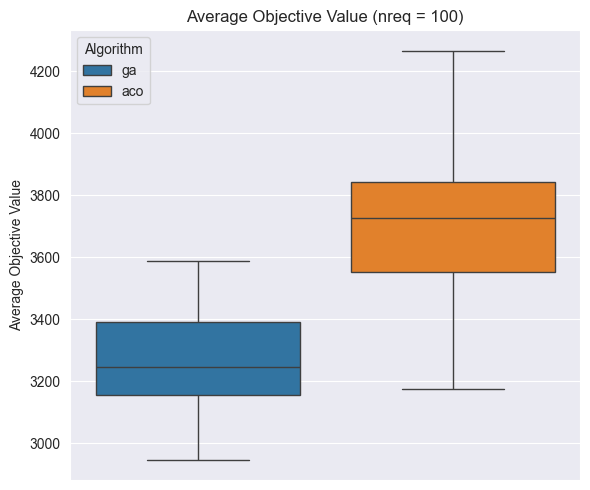
\includegraphics[width=0.42\linewidth]{graphics/comparison_ga_aco_100_obj.png}
    \hfill
    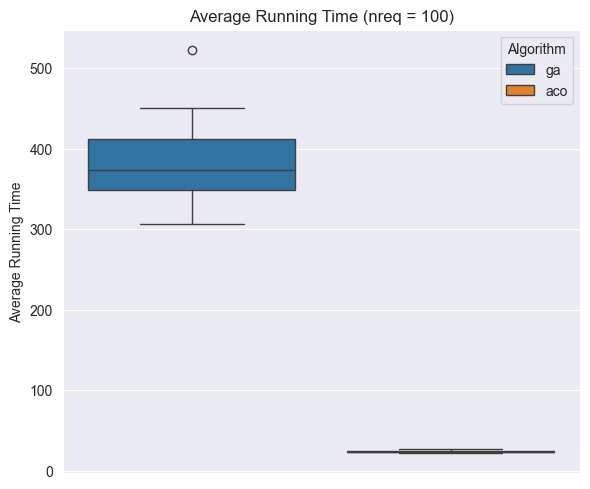
\includegraphics[width=0.42\linewidth]{graphics/comparison_ga_aco_100_time.png}
    \caption{Comparison GA vs. ACO: Average Objective Function and Run Time for
100 Customers}
    \label{fig:comparison_ga_aco_100}
\end{figure}

\begin{figure}[H]
    \centering
    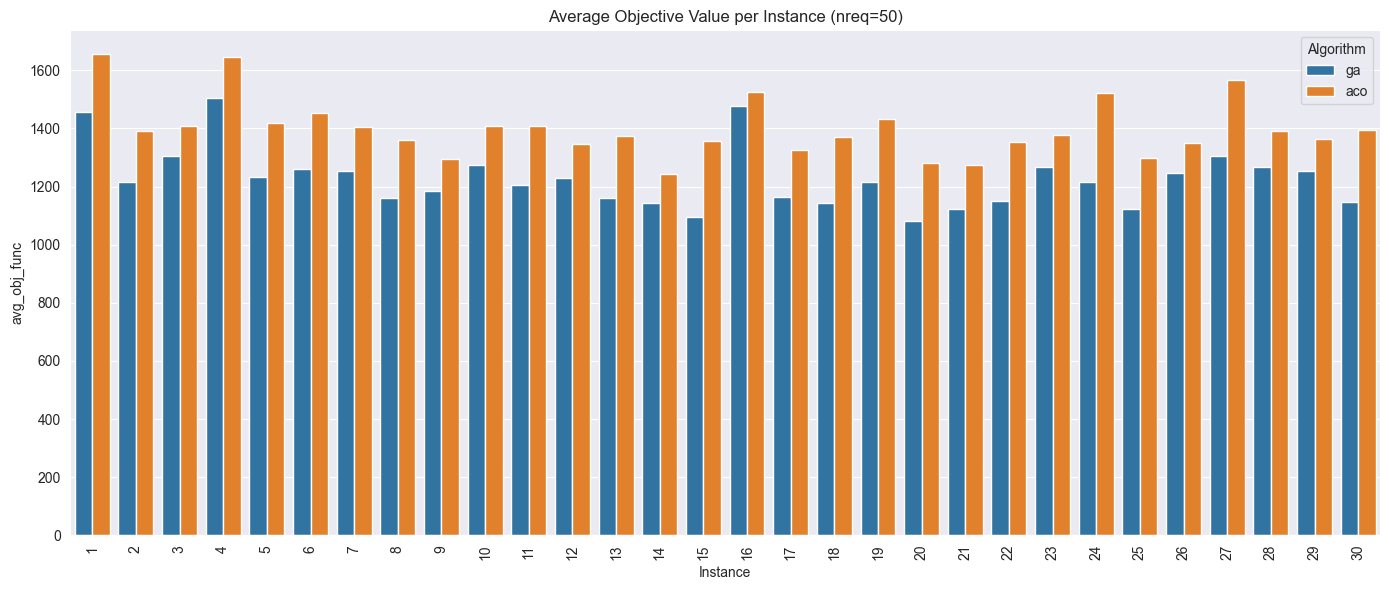
\includegraphics[width=0.95\linewidth]{graphics/comparison_ga_aco_50_obj_per_instance.png}
    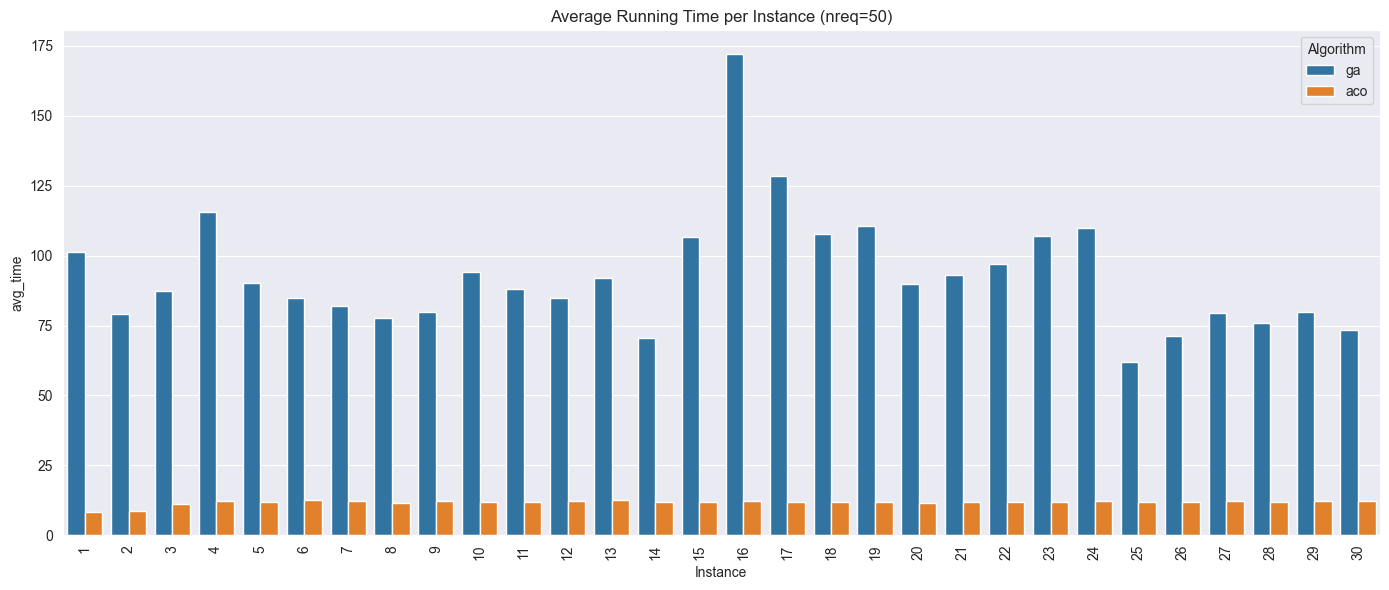
\includegraphics[width=0.95\linewidth]{graphics/comparison_ga_aco_50_time_per_instance.png}
    \caption{Comparison GA vs. ACO: Average Objective Function and Run Time for
50 Customers per Instance}
    \label{fig:comparison_ga_aco_50_per_instance}
\end{figure}

\begin{figure}[H]
    \centering
    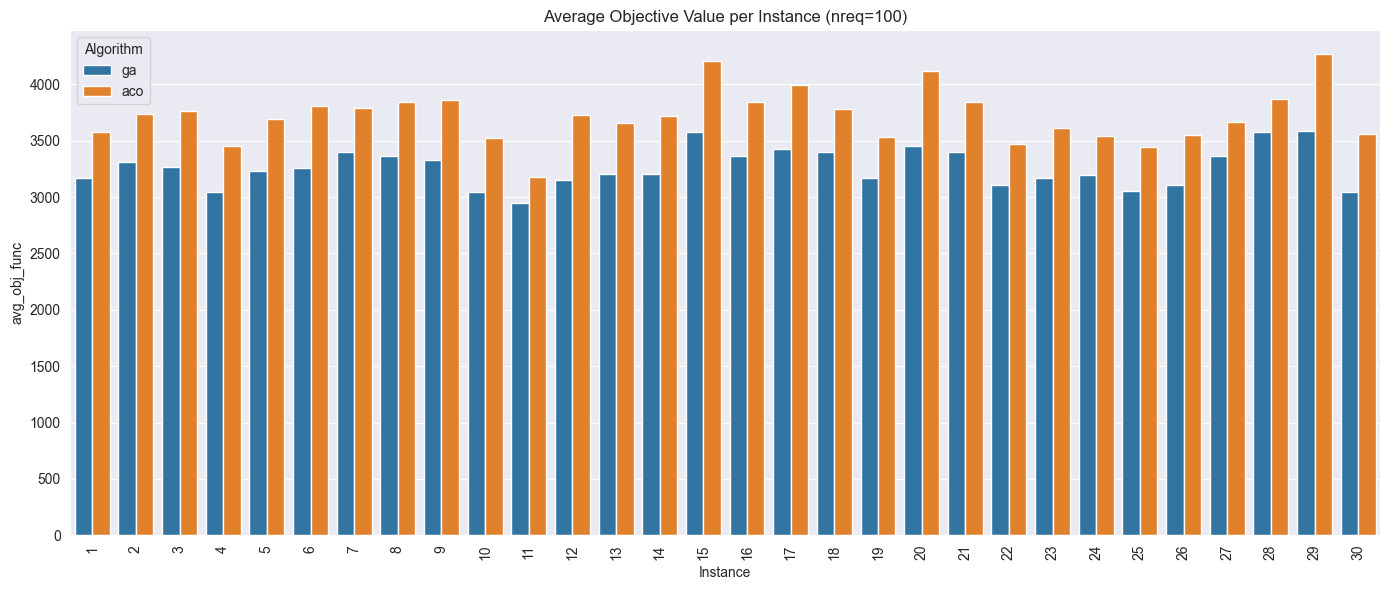
\includegraphics[width=0.95\linewidth]{graphics/comparison_ga_aco_100_obj_per_instance.png}
    \hfill
    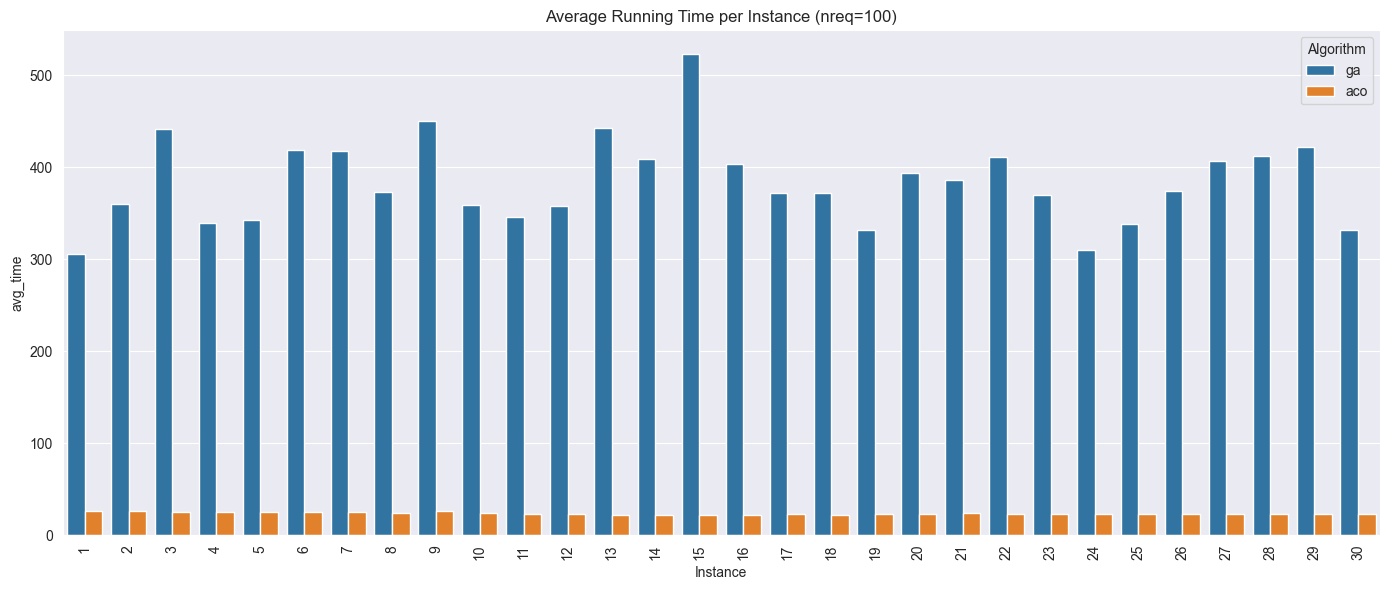
\includegraphics[width=0.95\linewidth]{graphics/comparison_ga_aco_100_time_per_instance.png}
    \caption{Comparison GA vs. ACO: Objective Function and Run Time for
100 Customers per Instance}
    \label{fig:comparison_ga_aco_100_per_instance}
\end{figure}

\subsubsection{Statistical Validation}

To formally verify this observation, a one-sided Wilcoxon signed-rank test was
applied using the following hypotheses:

\[
H_0: \text{GA} \ge \text{ACO} \quad \text{vs} \quad
H_1: \text{GA} < \text{ACO}.
\]

Tests were conducted separately for $nreq=50$ and $nreq=100$ with a significance
level of $\alpha = 0.05$.

\begin{table}[h]
\centering
\caption{One-sided Wilcoxon test: GA better than ACO}
\label{tab:one_ga_aco}
\begin{tabular}{c c c c}
\hline
$nreq$ & $W$ & $p$-value & Conclusion \\
\hline
50  & 0 & $9.31 \times 10^{-10}$ & GA significantly better \\
100 & 0 & $9.31 \times 10^{-10}$ & GA significantly better \\
\hline
\end{tabular}
\end{table}

For both problem sizes, the test statistic $W=0$ indicates that GA achieves lower
objective values than ACO on all paired instances. The extremely small p-values
provide overwhelming statistical evidence that GA outperforms ACO in terms of
solution quality.

\subsection{Comparison Between GA and VND}

After identifying GA as superior to ACO in terms of solution quality, GA is compared with VND, which was the best performing algorithm of the previous exercise.

\subsubsection{Experimental Results}

The experimental analysis shows that VND generally achieves lower objective
values than GA for both $nreq=50$ and $nreq=100$. This trend is visible in the
boxplots (Figures~\ref{fig:comparison_vnd_ga_50} and \ref{fig:comparison_vnd_ga_100}) and per-instance bar charts (Figures~\ref{fig:comparison_vnd_ga_50_per_instance} and \ref{fig:comparison_vnd_ga_100_per_instance}). For $nreq=100$, VND dominates GA on almost
all instances, while for $nreq=50$ only a small number of instances favor GA.

For the smaller instances ($nreq=50$), VND exhibits superior efficiency, converging significantly faster than GA. However, this trend reverses for the larger instances ($nreq=100$). While the execution time of GA is artificially constrained by a fixed computational budget (a 10-minute time limit), VND’s running time scales more aggressively with the problem size. Consequently, for $nreq=100$, VND becomes the more computationally intensive approach, whereas GA remains bounded by the predefined time threshold. This suggests that while VND achieves higher solution quality, it does so at the cost of significantly higher temporal requirements in larger search spaces.

\begin{figure}[H]
    \centering
    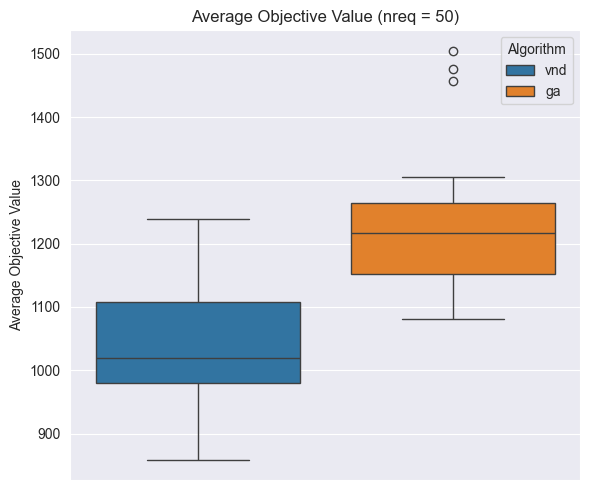
\includegraphics[width=0.42\linewidth]{graphics/comparison_vnd_ga_50_obj.png}
    \hfill
    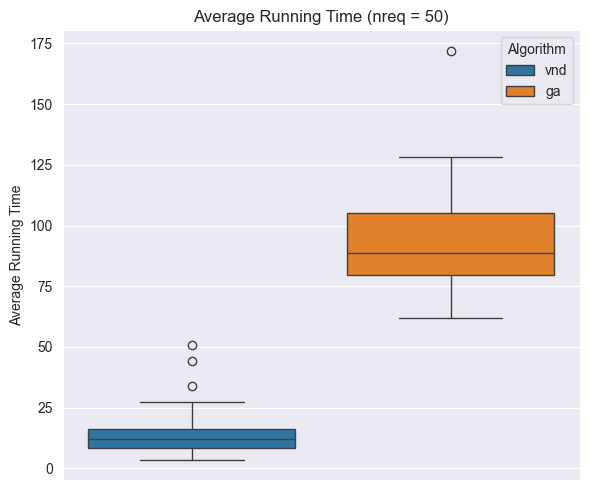
\includegraphics[width=0.42\linewidth]{graphics/comparison_vnd_ga_50_time.png}
    \caption{Comparison VND vs. GA: Average Objective Function and Run Time for
50 Customers}
    \label{fig:comparison_vnd_ga_50}
\end{figure}

\begin{figure}[H]
    \centering
    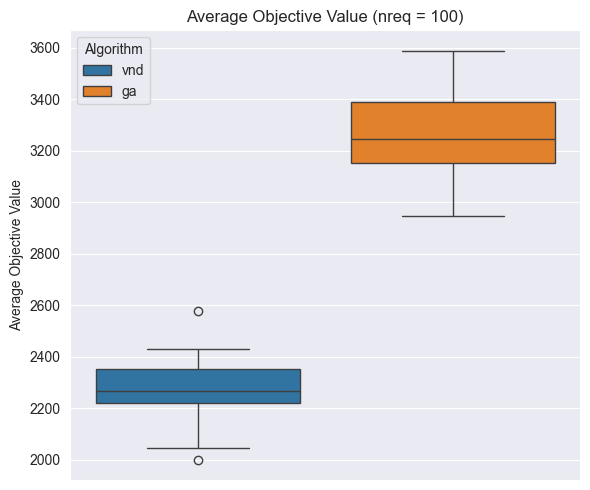
\includegraphics[width=0.42\linewidth]{graphics/comparison_vnd_ga_100_obj.png}
    \hfill
    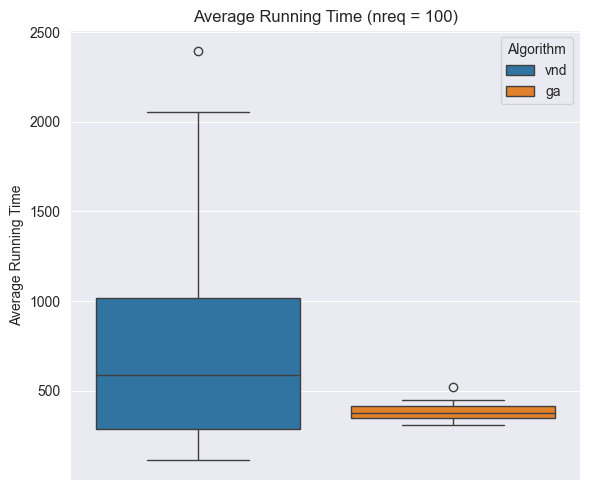
\includegraphics[width=0.42\linewidth]{graphics/comparison_vnd_ga_100_time.png}
    \caption{Comparison VND vs. GA: Average Objective Function and Run Time for
100 Customers}
    \label{fig:comparison_vnd_ga_100}
\end{figure}

\begin{figure}[H]
    \centering
    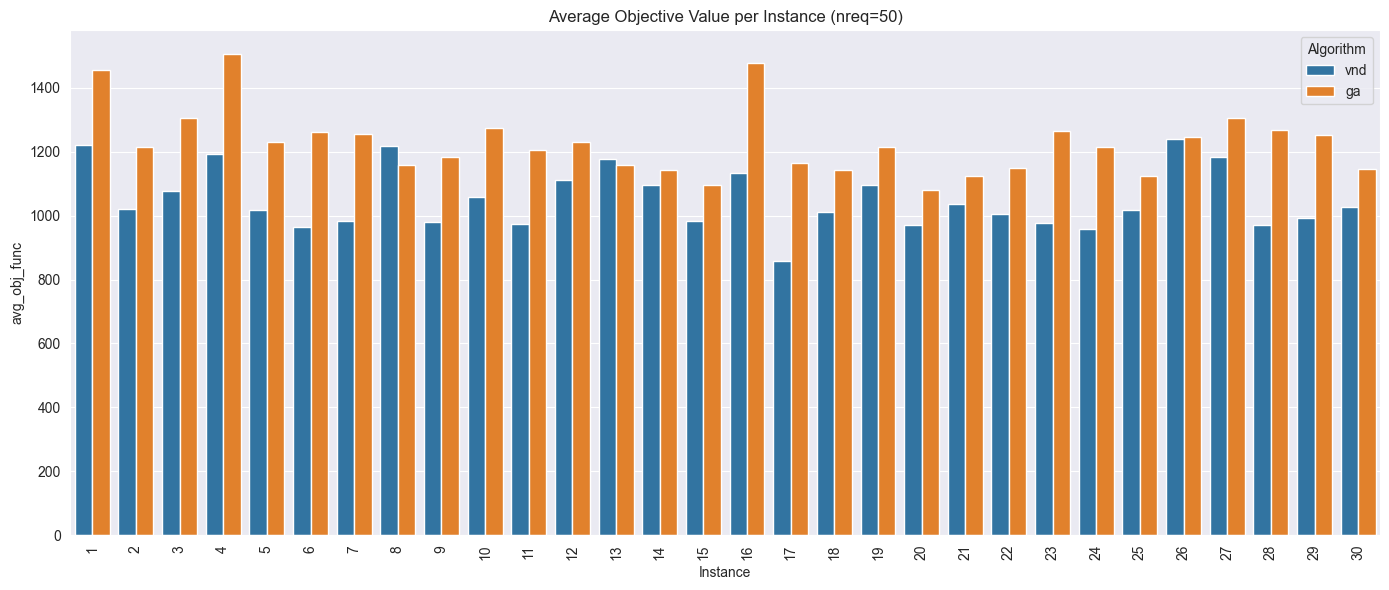
\includegraphics[width=0.95\linewidth]{graphics/comparison_vnd_ga_50_obj_per_instance.png}
    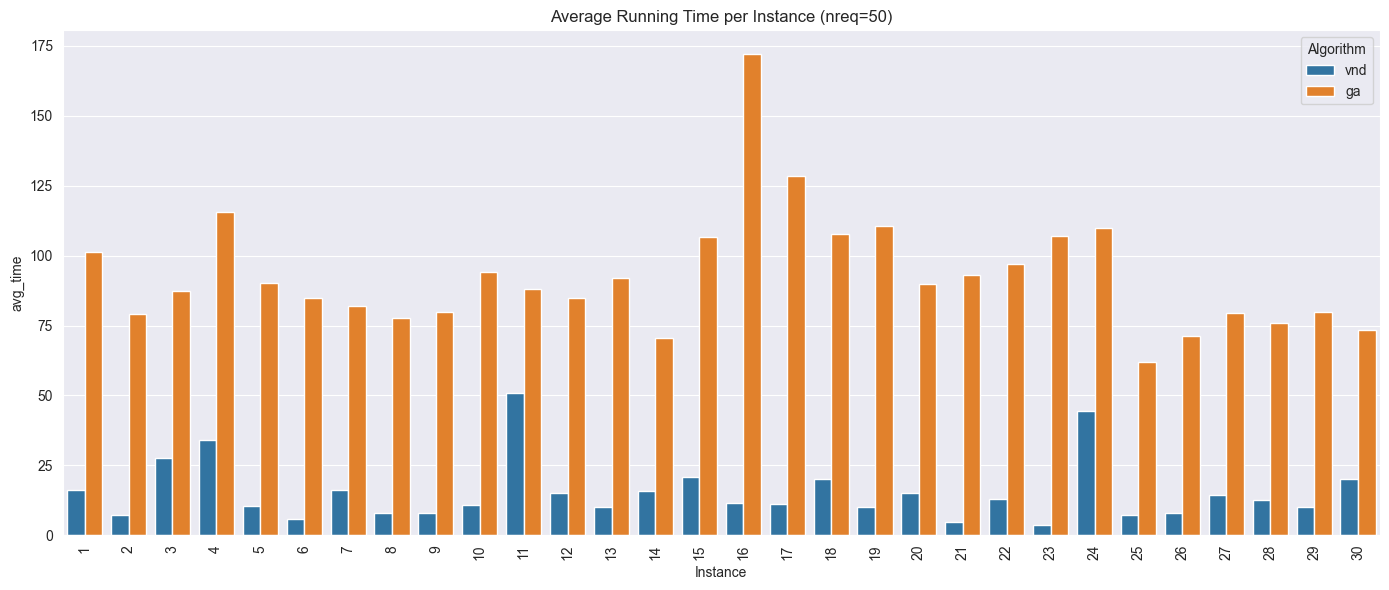
\includegraphics[width=0.95\linewidth]{graphics/comparison_vnd_ga_50_time_per_instance.png}
    \caption{Comparison VND vs. GA: Average Objective Function and Run Time for
50 Customers per Instance}
    \label{fig:comparison_vnd_ga_50_per_instance}
\end{figure}

\begin{figure}[H]
    \centering
    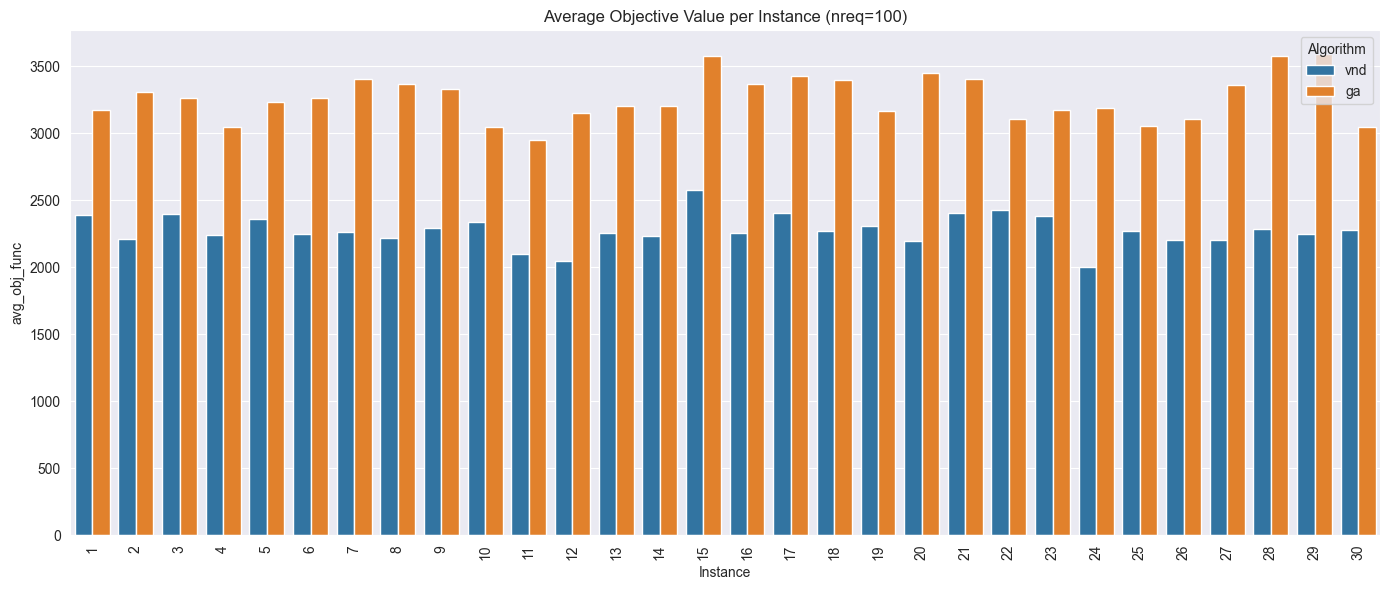
\includegraphics[width=0.95\linewidth]{graphics/comparison_vnd_ga_100_obj_per_instance.png}
    \hfill
    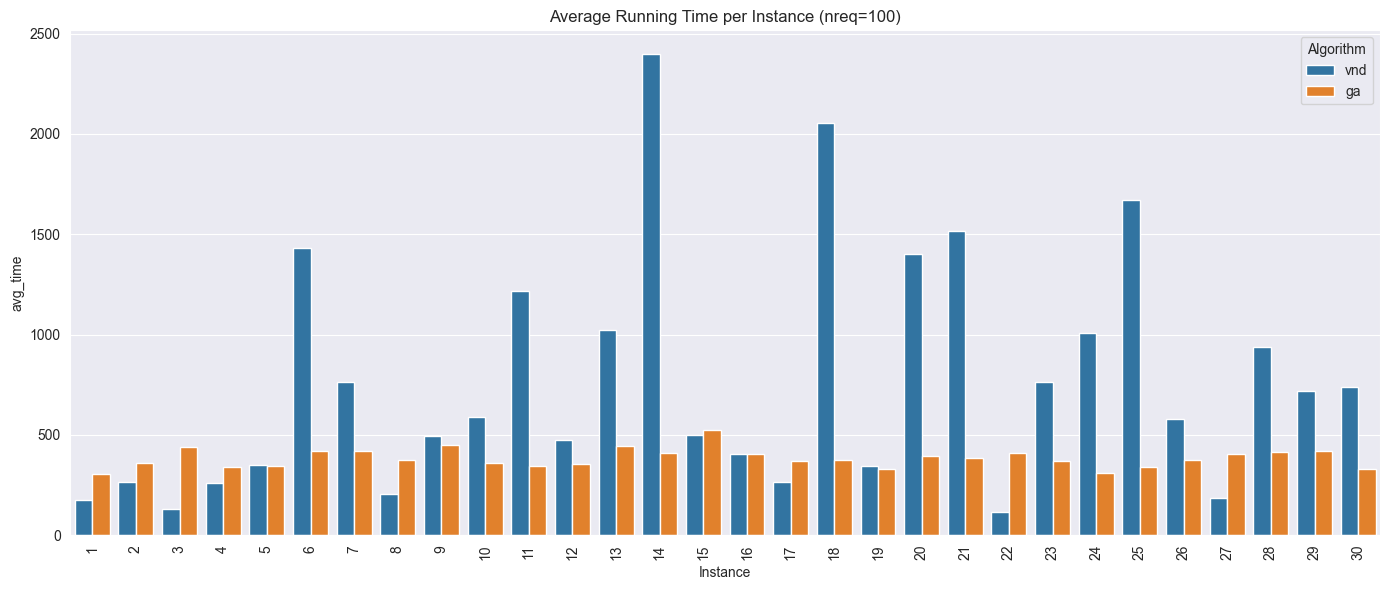
\includegraphics[width=0.95\linewidth]{graphics/comparison_vnd_ga_100_time_per_instance.png}
    \caption{Comparison VND vs. GA: Objective Function and Run Time for
100 Customers per Instance}
    \label{fig:comparison_vnd_ga_100_per_instance}
\end{figure}

\subsubsection{Statistical Validation}

To validate these observations, a one-sided Wilcoxon signed-rank test was
performed with the following hypotheses:

\[
H_0: \text{VND} \ge \text{GA} \quad \text{vs} \quad
H_1: \text{VND} < \text{GA}.
\]

Again, tests were conducted for $nreq=50$ and $nreq=100$ using $\alpha = 0.05$.

\begin{table}[h]
\centering
\caption{One-sided Wilcoxon test: VND better than GA}
\label{tab:one_vnd_ga}
\begin{tabular}{c c c c}
\hline
$nreq$ & $W$ & $p$-value & Conclusion \\
\hline
50  & 6 & $1.30 \times 10^{-8}$ & VND significantly better \\
100 & 0 & $9.31 \times 10^{-10}$ & VND significantly better \\
\hline
\end{tabular}
\end{table}

For $nreq=50$, a small number of instances favor GA, resulting in $W=6$, but the
p-value remains extremely small. For $nreq=100$, VND produces lower objective
values than GA on all instances ($W=0$). In both cases, the one-sided Wilcoxon
test confirms that VND significantly outperforms GA in terms of solution
quality.



\end{document}